\chapter{Nebenresultate}\label{chap:nebenresultat}

\section{Echter Rand}
    In einer ersten Annäherung an die \strukt, wurden Raumregionen als beliebige Teilmengen mit nichtleerem Inneren des $\R^3$ eingeführt, Flächenregionen als Mengen auf deren Rändern usw.
    Diese Mengen können niederdimensionale Ausläufer und Löcher haben, die im Sinne von $\theoryBSO$ nicht als räumliche Grenzen gelten sollten. 
    Der hier vorgestellte Ansatz arbeitet deshalb mit dem Begriff der einfachen Menge. 
    In einer früheren Version wurde dieses Problem durch den Begriff des echten Randes gelöst.
    Für einfache Mengen entspricht er dem topologischen Rand.

    \begin{dfn}[Echter Randoperator, echter Rand]\label{def:echtR} \ \vspace{8pt}

        \noindent
        Sei $X$ ein topologischer Raum. Dann ist der \textbf{echte Randoperator} $\Delta_X : 2^X \to 2^X$ definiert durch
    %	
        \begin{align*}
            \Delta_X := \rand_X \circ \co_X.
        \end{align*}
    %	
        Für eine Teilmenge $A \subseteq X$ heißt $\Delta_X(A)$ der \textbf{echte Rand} von $A$. Wenn eine Verwechslung mit anderen Topologien ausgeschlossen ist, schreiben wir auch $\Delta$.
        
    \end{dfn}

    \begin{satz} \label{satz:dco=doc} \ \vspace{8pt}

        \noindent
        Seien $X$ ein topologischer Raum, $A \subseteq X$. Dann gilt
        \begin{align*}
            \Delta(A) = \co(A) \setminus \oc(A) = \rand \circ \oc(A)
        \end{align*}
        (Beweis siehe \ref{anh:doc=doc})
    \end{satz}
    
    
\section{Kaskadierter Randoperator}\label{sec:kaskadierter-ro}
    Lange Zeit wurde der Ansatz verfolgt, eine ganze Familie von Interpretationen für $\theoryBSO$ zu definieren (siehe hierzu auch \ref{sec:offene-fragen}).
    Einer der Parameter dieser Familie war der zugrundgelegte Randbegriff.
    Da sich dieser für Raumregionen, euklidischen Flächen und euklidischen Linien definiert werden muss, wurde als allgemeinste Definition der kaskadierte Randoperator eingeführt.
    Er baut auf den Begriff des relevanten Randoperators auf.
    das ist ein Randoperator, der sich zwischen den Grenzfällen des echten und des äußeren Randes bewegt.
    
        \begin{dfn}[Relevanter Randoperator]\label{dfn:relevanter-rand} \ \vspace{8pt}

        \noindent
        Sei $X$ ein topologischer Raum.
        Ein relevanter Randoperator ist eine Abbildung $\rho: 2^X \to 2^X$ mit
        $$ \delta A \subseteq \rho(A) \subseteq \Delta A. $$
        Statt $\rho(A)$ schreiben wir auch $\rho A$
    \end{dfn}
    
    
    \begin{dfn}[Kaskadierter Randoperator in $\R^3$] \ \vspace{8pt}

        \noindent
        Sei $\rho: 2^{\R^3} \to 2^{\R^3}$ ein relevanter Randoperator auf $\R^3$.\\
        Für jedes beliebige $A \in \CO(\R^3)$ sei $\rho_A : 2^{\rho A} \to 2^{\rho A}$ ein relevanter Randoperator auf $\rho A$.\\
        Für jedes beliebige $A \in \CO(\R^3)$ und jedes beliebige $B \in \CO(\rho A)$ sei $\rho_{A,B} : 2^{\rho_A B} \to 2^{\rho_A B}$ ein relevanter Randoperator auf $\rho_A B$.\\
        Wir definieren folgende Mengen:
        \begin{align*}
            \mathcal{S}^3 &:= \CO(\R^3) \\
            \mathcal{S}^2 &:= \{(A,B) \mid A \in \mathcal{S}^3, B \in \CO(\rho A)\} \\
            \mathcal{S}^1 &:= \{(A,B,C) \mid (A,B) \in \mathcal{S}^2, C \in \CO(\rho_A B)\} \\
            \mathcal{S}^0 &:= \{(A,B,C,D) \mid (A,B,C) \in \mathcal{S}^1, D \in \CO(\rho_{A,B} C)\}\\
            \mathcal{S} &:= \mathcal{S}^3 \cup \mathcal{S}^2 \cup \mathcal{S}^1 \cup \mathcal{S}^0
        \end{align*}
        Definiere dann die Funktion $b : \mathcal{S} \to 2^{\R^3}$ über
        \begin{itemize}
            \item $b(A) = \rho A$ für $A \in \mathcal{S}^3$
            \item $b(A,B) = \rho_A B$ für $(A,B) \in \mathcal{S}^2$
            \item $b(A,B,C) = \rho_{A,B} C$ für $(A,B,C) \in \mathcal{S}^1$
            \item $b(A,B,C,D) = \varnothing$ für $(A,B,C,D) \in \mathcal{S}^0$
        \end{itemize}
        %
        Jede so konstruierte Funktion ist ein \textbf{kaskadierter Randoperator}.
    \end{dfn}
    

\section{Lokaler Zusammenhang}\label{sec:lok-zusammenhang}

    In Abbildung \ref{fig:zusammenhang} ist 
    %im Beispiel zu $1$-dimensional zusammenhängenden Flächenregionen 
    eine lokal $0$-dimensional zusammenhängenden Flächenregion dargestellt.
    Diese Idee des lokalen Zusammenhangs entstammt ursprünglich einer Diskussion zu dem in [\cite{baumann-r-2019--a}] eingeführten Begriff der Continuousness.

    Er hat jedoch noch eine weitere Relevanz für die Modellbildung die in \ref{sec:offene-fragen} thematisiert wurde:
    An solchen Stellen, an denen eine Raumentitäten lokal weniger stark zusammenhängt ist ihr Rand in der \strukt keine Mannigfaltigkeit.
    Dies bringt möglicherweise Probleme mit sich bei der Untersuchung der Dimension des Randes einer solchen Entität.

    Lokaler Zusammenhang lässt sich im Rahmen der $\theoryBS$-Theorie definieren, ist aber in der \strukt einfacher zu verstehen, weshalb ich diese Definition hier voranstellen möchte.
    Da ich parallel mit Symbolen aus $\theoryBSO$ als auch aus der \strukt arbeite, unterscheide ich die Struktur-Symbole durch ein hochgestelltes $\mathcal{O}$.

    Eine Raumregion $A$ ist lokal $0$-dimensional zusammenhängend im Punkt $y$ im Rand von $A$, wenn es ein $\varepsilon < 0$ gibt, so dass für alle $\eta < \varepsilon$ die Raumregion $\ball_{\eta}(y) \cap A$ $0$-dimensional, aber nicht $1$-dimensional zusammenhängend ist. Siehe hierzu Abbildung \ref{fig:loc0dc}.
    
    \begin{figure}[ht]
        \centering
        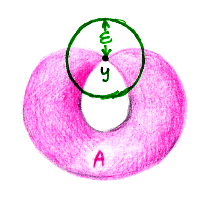
\includegraphics[height=4cm]{abb/loc0dc.png}
        \caption{Beispiel für eine lokal $0$-dimensional zusammenhängende Raumregion}
        \label{fig:loc0dc}
    \end{figure}
    
    In ähnlicher Weise wird dieser Begriff für Flächenregionen und für lokal $1$-dimensional zusammenhängende Raumregionen definiert.

    \begin{dfn}[Lokal 0/1-zusammenhängend in der \strukt]\ \vspace{0pt}

        \begin{itemize}
            \item Eine Raumregion $A$ ist lokal $0$-dimensional zusammenhängend im Punkt $[A', B', C', \{y\}]$, wenn gilt
            \begin{align*}
                &\Stangpart([A', B', C', \{y\}],A) \land \exists \varepsilon \forall \eta: (\eta < \varepsilon \to 
                \\
                &\SzeroDC(\ball_{\eta}(y) \cap A) \land \neg \SoneDC(\ball_{\eta}(y) \cap A))
            \end{align*}
            \item Eine Flächeregion $[A,B]$ ist lokal $0$-dimensional zusammenhängend im Punkt $[A', B', C', \{y\}]$, wenn gilt
            \begin{align*}
                &\Stangpart([A', B', C', \{y\}],[A,B]) \land \exists \varepsilon \forall \eta:
                %\\
                (\eta < \varepsilon \to
                \\
                &\SzeroDC([A,\ball_{\eta}(y) \cap B]) \land \neg \SoneDC([A,\ball_{\eta}(y) \cap B]))
            \end{align*}
            \item Eine Raumregion $A$ ist lokal $1$-dimensional zusammenhängend im Punkt $[A', B', C', \{y\}]$, wenn gilt
            \begin{align*}
                &\Stangpart([A', B', C', \{y\}],A) \land \exists \varepsilon \forall \eta: (\eta < \varepsilon \to 
                \\
                &\SoneDC(\ball_{\eta}(y) \cap A) \land \neg \StwoDC(\ball_{\eta}(y) \cap A))
            \end{align*}
        \end{itemize}
        
    \end{dfn}
%     
    Da es in $\theoryBS$ keinen Abstandsbegriff gibt, lässt sich diese Definition nicht so ohne weiteres auf die Theorie hochziehen. 
    In $\theoryBS$ definiere ich den lokalen Zusammenhang auf folgende Weise:
%
    \begin{dfn}[$x$ ist lokal $0$/$1$-dimensional zusammenhängend in $y$]
        \begin{align*}
            \Gloczerodc(x,y) := &\GzeroD(y) \land \Gtangpart(y,x) \land
                                \\
                                &\exists u\ (\forall v w\ (\Ginpart(y,v) \land \Gspart(v,u) \land
                                \\
                                &\Gintersect(x,v,w) \to \neg \GoneDC(w)))
                                \\
            \Gloconedc(x,y) := &\neg \Gloczerodc(x,y) \land \GzeroD(y) \land \Gtangpart(y,x) \land
                                \\
                                &\exists u\ (\forall v w\ (\Ginpart(y,v) \land \Gspart(v,u) \land
                                \\
                                &\Gintersect(x,v,w) \to \neg \GtwoDC(w)))
        \end{align*}

    \end{dfn}
%
    Es ist noch zu zeigen, dass beide Definitionen kompatibel sind.
    Abbildung \ref{fig:loc1dc} zeigt ein Beispiel einer lokal $1$-dimensional zusammenhängenden Raumregion.

    \begin{figure}[ht]
            \centering
            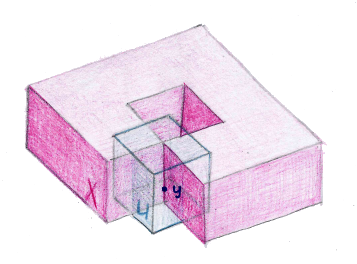
\includegraphics[width=0.6\textwidth]{abb/loc1dc.png}
            \caption[Beispiel für eine lokal $1$-dimensional zusammenhängende Raumregion]{Beispiel für eine lokal $1$-dimensional zusammenhängende Raumregion: $x$ ist lokal $1$-dimensional zusammenhängend in $y$, da es eine Umgebung $u$ von $y$ gibt, der keinen Teil hat, der auch eine Umgebung von $y$ ist und dessen Schnitt mit $x$ $2$-dimensional zusammen hängt.}
            \label{fig:loc1dc}
    \end{figure}
